

\documentclass{article} 
\usepackage{todonotes}
\usepackage{graphicx}
\usepackage{grffile}
\usepackage{algorithm}
\usepackage[noend]{algpseudocode}
\usepackage{float}
\usepackage[font=footnotesize,labelfont=bf]{caption}
\usepackage[left=0.8in, right=0.8in, top=0.9in, bottom=1in]{geometry}
\usepackage{hyperref} 
%\usepackage{caption}
\graphicspath{ {images/} }


\title{ \textbf {\vspace{0.1cm}\Huge Parallel Jacobi\\ \vspace{0.3cm}}
 Final Project for the SPM course \vspace{0.5cm}\\} 

\date{\vspace{1.0cm}}

\author{ \Large Francesco Balzano \vspace{0.3cm}\\ 
%Matricola 541533 \vspace{0.5cm}\\
\Large Master Degree in Computer Science and Networking \vspace{0.4cm} \\
\Large A.Y. 2016-2017 
}


\begin{document}
  \pagenumbering{gobble}
  \maketitle
  %\newpage
  \noindent\rule{18cm}{0.4pt}
  \tableofcontents
  \newpage
  \pagenumbering{arabic}

\clearpage
\setcounter{page}{2}
  
\section{Problem}
Write a parallel application that finds the solution of a system of linear equations using the Jacobi iterative method. 
\section{Dependency analysis} \label{dep_an}
The algorithm iterates until either the maximum number of iterations is reached or a stopping condition occurs (\textit{e.g.} a convergence condition). \\
Basically, at each iteration the algorithm computes the following equations:
\[
\left\{ 
\begin{array}{c}
\sigma\textsubscript{i} = \displaystyle\sum_{j \neq i}^{} A_{i,j} \: X_{j}^{(k)}       \\
X_{i}^{(k+1)}  = \frac{1}{A_{i,i}} (b_{i} - \sigma\textsubscript{i})                    \\ 
\end{array}
\right. 
\]

$\forall i = 1, ... , n $. \\ \\
Unfortunately, the two equations cannot be parallelized because they violate the Bernstein conditions. Indeed, if we consider the same iteration of the algorithm, a \textit{READ-AFTER-WRITE} dependency holds for $\sigma\textsubscript{i}$. We cannot even parallelize the second equation at step \textit{K} and the first equation at step \textit{K+1}, because in that case it holds a \textit{READ-AFTER-WRITE} dependency on $X$. So $X_{i}^{(k+1)}$ can be started to be computed only after $X_{i}^{(k)}$ has been computed. 

\begin{figure}[h]
\centering
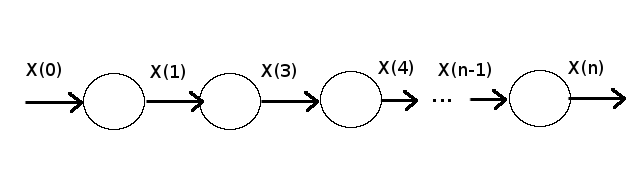
\includegraphics[scale=0.43]{dependency_chain}
\caption{Chain of dependencies}
\label{fig:dep_chain}
\end{figure}     

\section{Decomposition strategies}
I analyze some alternative strategies to turn the problem into a set of concurrent activities. Each alternative is characterized by a different level of granularity for the concurrent activities. In this section the main metric kept into account to conduct the assessment of the alternatives is the \textit{Completion Time} $T_{C}$, because the computation is a \textit{data parallel} one. Besides, the completion time refers to the single iteration of the Jacobi iterative method. In the following, I am assuming that the concurrent activities are instantiated inside a loop run on a single processing element, so the time to setup them is fully paid. Instead, once setup they can (possibly) run in parallel, and so when assessing the completion time I consider the slowest path in the concurrency graph that must be serialized. In the following formulas I indicate with $T_{aritm}$ the time neeeded to perform an aritmetic operation. This is a big semplification, introduced to keep more compact and readable the formula. The rationale is that any aritmetic operation takes $O(10^{-9})s$, so I use $T_{aritm}$ and $O(10^{-9})s$ as synonyms. Furthermore I introduce $T_{comm}$ to express the communication time. $T_{comm}(1)$ will be used when the amount of data sent is constant.    

\subsection{Tree of concurrent activities}
We can decompose the concurrent activities in a tree made of n independent subtrees. Based on the kind of computation done, we can recognize three different types of concurrent activities: 
\begin{itemize}
\item \textit{Leaves:} Each leaf receives $A_{i,j}$ and $X_{j}^{(k)}$ and computes $A_{i,j} * X_{j}^{(k)}$; 
\item \textit{Internal nodes:} Each internal node receives two quantities (one from each son), makes the sum and passes it to its father in the tree. 
\item \textit{Roots(of the n subtrees):} The $i^{th}$ root receives two quantities from its sons, makes their sum to finish the computation of $\sigma\textsubscript{i}$ and then computes $X_{i}^{(k+1)}$.    
\end{itemize}

\paragraph{Performance model} To deduce the performance model I consider for a moment the implementation of the concurrent activities. The details will be discussed later, but for the moment being I notice that the concurrent activities will be eventually mapped into processing elements. If I map each of these concurrent activities into a distinct processing element I have a waste of resources, because at any time a significant fraction of them will be idle. What I can do instead, is to map both internal nodes and roots into the processing elements that were used to run the leaves. Let us call \textit{Workers} the leaves of the tree: then we are mapping the tree of concurrent activities into the array of workers $[W_{1,2},W_{1,3}, ... ,W_{n,n-1}]$ . \\

\begin{figure}[h]
\centering
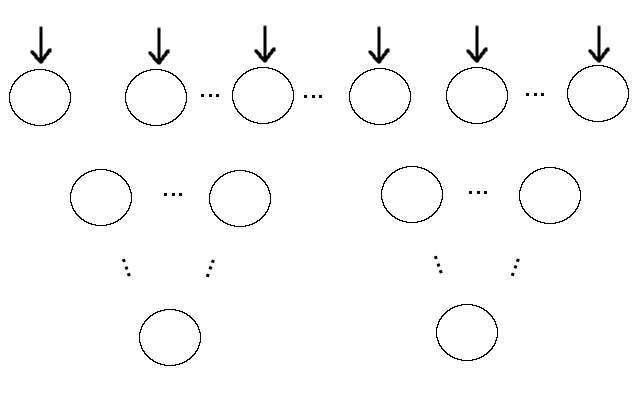
\includegraphics[scale=0.48]{tree_ca}
\caption{Decomposition strategy number 1: tree of workers}
\label{fig:tree_ca}
\end{figure} 

\begin{itemize}
\item \textbf{Number of Workers:} $O(n^2)$
\item \textbf{Height(tree):} $O(\log n)$. Indeed the tree is made of n, independent subtrees, without cross edges between different subtrees. Each subtree is a complete binary tree with \textit{n-1} leaves.
\item Each level of the tree can be computed in parallel
\item \textbf{Completion Time:} $T_{C} = O(n^2) \: T_{setup} + O( \log n) \: (T_{calc} + T_{comm}(1) ) = O(n^2) \: T_{setup} + O( \log n) \: (T_{aritm} + T_{comm}(1) )$. Since each concurrent activity makes a constant number of aritmetic operations, it's calculation time is modelled by $T_{aritm}$. The overhead of this decomposition strategy is given by the time to setup the concurrent activities ($O(n^2) \: T_{setup}$) and by the communication of intermediate results through the levels of the tree ($O( \log n) \: T_{comm}(1$)).
\end{itemize}


\subsection{Array of concurrent activities}
Each worker $W_{i}$ receives $A_{i,*}$ and $X^{k}$ and computes $X_{i}^{(k+1)}$, \textit{i.e.} it computes the system of section \ref{dep_an} for some $i \in {1,2, ... , n}$ This strategy corresponds to collapse each independent subtree of figure \ref{fig:tree_ca} into a single worker.
\paragraph{Performance model} 

\begin{figure}[h]
\centering
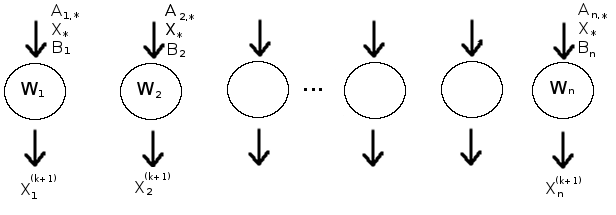
\includegraphics[scale=0.48]{array_ca}
\caption{Decomposition strategy number 2: array of workers}
\label{fig:array_ca}
\end{figure} 

\begin{itemize}
\item \textbf{Number of Workers:} $n$
\item \textbf{Completion Time:} $T_{C} = O(n) \: T_{setup} + T_{calc} + T_{comm}(1) = O(n) \: T_{setup} + O(n) \: T_{aritm} + T_{comm}(1)$. The calculation time $T_{calc}$ of each concurrent activity is modelled by $O(n) \: T_{aritm}$, because each Worker makes approximately $O(n)$ sums and $O(n)$ multiplications. The overhead of this decomposition strategy is basically given by the time to setup the n concurrent activities, which is $O(n) \: T_{setup}$.
\end{itemize}

\subsubsection{Array of concurrent activities with pipeline}
Since the computation of the worker in the decomposition number two takes a time linear and not constant, we could try to lower the service time by inserting a 2-stage pipeline. In this new parallelization, the first stage of the pipeline that parallelizes $W_i$ computes $\sigma\textsubscript{i}$, while the second stage computes $X_{i}^{(k+1)}$. We are forced to build this exact configuration of the pipeline because we must keep into account the data dependencies already pointed out in section \ref{dep_an}.\\ 
\paragraph{Performance model} This parallelization is not worth it, because stage one takes $O(n) \: T_{aritm}$ while stage 2 takes $O(1) \: T_{aritm}$, so if there is a bottleneck in decomposition number two we are not able to remove it with this parallelization. Furthermore a pipeline may reduce the service time but increases the latency, and since we are more interested in completion time than throughput we don't find it very useful    . \\

\begin{figure}[h]
\centering
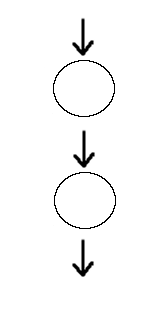
\includegraphics[scale=0.48]{single_worker_pipe}
\caption{Decomposition strategy number 2, variant with pipeline: only the first worker is considered}
\label{fig:w_pipe}
\end{figure} 

\subsection{Shortened tree of concurrent activities}
We have already said that we can see the array of concurrent activities as a tree of concurrent activities in which each subtree has been collapsed into a single concurrent activity. These are the two extreme situations, but we can also consider an intermediate situation in which each subtree is implemented with $O(1)$ workers and not with $O(n)$. Let us assume that the total number of workers is $m$, with $n \leq m \leq n^2$. 

\paragraph{Performance model}
\begin{itemize}
\item \textbf{Number of Workers:} $m$
\item \textbf{Height(tree):} $O(\log \frac{m}{n})$. Indeed the tree is made of n, independent, binary subtrees, each one having $O(\frac{m}{n})$ leaves.
\item \textbf{Completion Time:} $T_{C} = O(m) \: T_{setup} + \: O( \frac{n^2}{m}) \: T_{aritm} + O(\log \frac{m}{n})(T_{aritm} \: + \: T_{comm}(1)) )$. The contribute $O(m) \: T_{setup}$ is paid to setup the concurrent activities, $O( \frac{n^2}{m}) \: T_{aritm}$ is due to the leaves (which perform the most of the computations) and finally $O(\log \frac{m}{n})(T_{aritm} \: + \: T_{comm}(1)) )$ is for the internal nodes and the roots (they perform a constant number of arithmetical operations). \\ 
The nice thing of this decomposition is that it includes as special cases both decompositions one and two: indeed, if $m = O(n^2)$ than we get the completion time of decomposition one, whereas if $m = O(n)$ we get the completion time of decomposition two. 
\end{itemize}

\subsection{Single concurrent activitiy}
We consider a single worker $W$ that receives $A$ and $X$ and computes $X^{(k+1)}$, \textit{i.e.} it computes the system of section \ref{dep_an} $\forall i \in 1, ... , n $. .
\paragraph{Performance model} 

\begin{figure}[h]
\centering
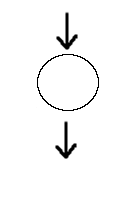
\includegraphics[scale=0.52]{single_worker_p3}
\caption{Decomposition strategy number 4: single worker}
\label{fig:worker}
\end{figure} 

\begin{itemize}
\item \textbf{Number of Workers:} $1$
\item \textbf{Completion Time:} $T_{C} = O(n^{2}) \: T_{aritm}$. If we instantiate the concurrent activity on a processing element different from the one running the main flow of control we should consider in principle also the time $O(1) \: T_{setup} + \: T_{comm}(n)$. Anyway this quantity can be neglected when compared to the shown completion time, especially if n is big.
\end{itemize}

\section{Evaluation}
In this section I carry out a theoretical evaluation of the alternative decomposition strategies based on their performance model. In order to conduct a quantitative evaluation of the alternatives I need some (approximated) value for $T_{comm}$ and $T_{setup}$. These value are architecture-dependent, and we target a shared-memory architecture. I assume $T_{comm}$ to be the time needed to access main memory, and based on the values found on Peter Norvig's site (\cite{access_time}) I assume $T_{comm} \: = \: O(10^{-7})s$. This is a semplification that does not keep into account that some data is shared among processing elements, and even in the favourable case in which the implementation is lock-free there is some overhead in the management of shared blocks. For instance, if some block is replicated in the caches of different processing elements, if one processing element modifies such block than a cache coherence protocol will be fired to keep the value of such block consistent among caches. In a shared-memory architecture $T_{setup}$ is the time to start a thread. Based on experimental values, I deduced that the time to start a thread should be approximately $O(10^{-5})s$. \\
Different decomposition strategies may be convenient for different data size. For this reason, I consider three different values for n: 100, 1000 and 10000.     

\hskip1.60cm
\renewcommand{\arraystretch}{2}
\begin{tabular}[c]{ |l|l| }
  \hline 
  \multicolumn{2}{|c|}{\textbf{Tree of concurrent activities}: $ T_C = O(n^2) \: T_{setup} + O( \log n) \: (T_{aritm} + T_{comm}(1) )$ } \\[10pt]
  \hline
  n = 100 & $T_C = (10^4 * 10^{-5} + 6,64 * (10^{-9} + 10^{-7}))s = O(10^{-1})s$ \\
   \hline
  n = 1000 & $T_C = (10^6 * 10^{-5} + O(10^{-7}))s = O(10)s$  \\
  \hline
  n = 10000 & $T_C = (10^8 * 10^{-5} + O(10^{-7}))s = O(10^3)s$ \\
  \hline 
\end{tabular} \\[15pt]

\hskip1.60cm
\renewcommand{\arraystretch}{2}
\begin{tabular}[c]{ |l|l| }
  \hline 
  \multicolumn{2}{|c|}{\textbf{Array of concurrent activities}: $ T_C = O(n) \: T_{setup} + O(n) \: T_{aritm}$ } \\[10pt]
  \hline
  n = 100 & $T_C = (10^2 * 10^{-5} + 10^2 * 10^{-9})s = O(10^{-3})s$ \\
   \hline
  n = 1000 & $T_C = (10^3 * 10^{-5} + 10^3 * 10^{-9})s = O(10^{-2})s$  \\
  \hline
  n = 10000 & $T_C = (10^4 * 10^{-5} + 10^4 * 10^{-9})s = O(10^{-1})s$ \\
  \hline 
\end{tabular} \\[15pt]

\hskip1.60cm
\renewcommand{\arraystretch}{2}
\begin{tabular}[c]{ |l|l| }
  \hline 
  \multicolumn{2}{|c|}{\textbf{Single concurrent activity}: $ T_C = O(n^2) \: T_{aritm}$ } \\[10pt]
  \hline
  n = 100 & $T_C = (10^4 * 10^{-9})s = O(10^{-5})s$ \\
   \hline
  n = 1000 & $T_C = (10^6 * 10^{-9})s = O(10^{-3})s$  \\
  \hline
  n = 10000 & $T_C = (10^8 * 10^{-9})s = O(10^{-1})s$ \\
  \hline 
\end{tabular} \\[15pt]
Looking at the tables above, we see that the solution with a single concurrent activity has the best performances. This strange result arises because we are considering too many concurrent activities. Indeed, if we look at the formulas in the first and second table, we can easily recognize that the bottleneck is the time to setup the concurrent activities (\textit{i.e.} the threads). The solution is thus instantiating a smaller number of concurrent activities, which will do coarser grain computations. Because I want to make coarser grain computations in order to achieve better performances, I abandon the decomposition with the tree (also the shortened version). I only consider the decomposition with the array of workers for the implementation. In order to make a check that this could be the right way, let's consider 100 concurrent activities computing one iteration of the Jacobi iterative method with n = 10000. We get:  
\[ T_C = 100 \: T_{setup} + O(\frac {n^2}{100}) \: T_{aritm} = (10^2 * 10^{-5} + 10^6 * 10^{-9})s = O(10^{-3})s \]  \\
that is the solution with the array made of 100 workers could be 100 times faster in computing the single iteration of the Jacobi method with respect to the sequential implementation. This is a result that comes from the assumption that the workers can do their job independently from one another. This could not be the case, for instance, if they need to read/write the data from/to the same place, their accesses could be serialized. 

\section{Implementation} 
I have implemented the Jacobi iterative method both in a sequential and in a parallel way. The sequential implementation is a simple single-threaded program. The parallel implementaion has been done both with pthreads and with fastflow. In the implemenation with pthreads I provide two alternatives: one using mutexes and condition variables, the other lock-free with busy waiting. In the implementation with fastflow, I have used the \textit{parallelFor} construct to run the concurrent activities in parallel.


I decided to implement the second decomposition strategy, because is the one that according to me ffers the best tradeoff ``Parallelism Degree VS Overhead''. In this section I describe the main points concerning implementation decisions. While in the previous section I considered a single iteration of the Jacobi method, now I take into account that it is an iterative method. \\
The problem is a \textbf{data parallel} one: so I can consider a \textbf{map} decomposition. I must take into account the following features:
\begin{itemize}
\item \textbf{Split} of the data to be sent to the workers. This is tipically done by a \textbf{scatter} process, that sends the appropriate partition to each Worker, but since:
	\begin{itemize}
	\item $W_{i}$ reads only $A_{i,*}$ and $X^{k}$ 
	\item $W_{i}$ writes $X_{i}^{(k+1)}$, but it is the \textit{only one} that makes such write
	\item I target a \textit{shared-memory} architecture.
	\end{itemize}
I avoid using a scatter process that sends to each Worker the partition of data on which it has to do the computation. Instead, I will merge the scatter and the gatherer process into a single processing element and will assign the appropriate partitions to each worker only once at creation time.
\item \textbf{Computation} done by each Worker $W_{i}$: at initialization time each worker is simply provided a reference to $A, X$ and $B$ and the index $i$. After the computation, it updates $X_{i}^{(k+1)}$ in memory and tells the scatter that it has completed the current iteration.
\item \textbf{Gathering} of the results: the \textbf{gatherer} process waits that all the $W_{i}$ have concluded the computation for the current iteration and then:
	\begin{itemize}
	\item either stop the Workers and output the final $X$;
	\item or notify all the Workers to go on with another iteration.
	\end{itemize}
As already pointed out, I merge the scatter and the gatherer into a single process. This allows me to save one processing element and to have a centralized ``Locus of Control'' to control the execution of the program. \\
\end{itemize}
So the structure of the chosen parallelization is basically a map without the gatherer.

\begin{figure}[h]
\centering
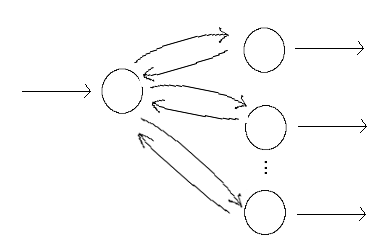
\includegraphics[scale=0.58]{map_no_g}
\caption{Structure of the implemented decomposition}
\label{fig:worker}
\end{figure} 


\begin{thebibliography}{9}
\bibitem{access_time} 
Peter Norvig. 
\textit{Teach Yourself Programming in Ten Years},\href{ 
http://norvig.com/21-days.html\#answers}http://norvig.com/21-days.html\#answers.
\end{thebibliography} 

\end{document}
